\documentclass[12pt, twoside]{article}
\usepackage[letterpaper, margin=1in, headsep=0.5in]{geometry}
\usepackage[english]{babel}
\usepackage[utf8]{inputenc}
\usepackage{amsmath}
\usepackage{amsfonts}
\usepackage{amssymb}
\usepackage{tikz}
\usetikzlibrary{quotes, angles}
\usepackage{graphicx}
\usepackage{enumitem}
\usepackage{multicol}

\newif\ifmeta
\metatrue %print standards and topics tags

\title{Regents Geometry}
\author{Chris Huson}
\date{December 2021}

\usepackage{fancyhdr}
\pagestyle{fancy}
\fancyhf{}
\renewcommand{\headrulewidth}{0pt} % disable the underline of the header
\raggedbottom


\fancyhead[LE]{\thepage}
\fancyhead[RO]{\thepage \\ Name: \hspace{4cm} \,\\}
\fancyhead[LO]{BECA / Dr. Huson / Geometry 04 Analytic Geometry}

\begin{document}

\subsubsection*{4.16 Review: Triangle angles}
\begin{enumerate}
  \item Do Now: Given isosceles $\triangle LMN$, $\overline{LM} \cong \overline{NM}$. If $m\angle L=4x+19$ and $m\angle N=7x-8$, find $m\angle M$.
  \begin{flushright}
  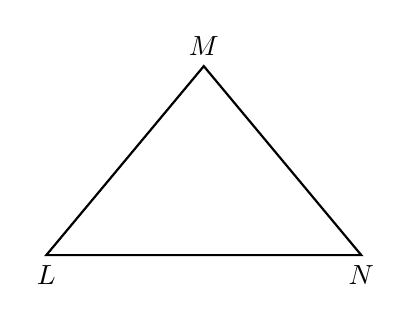
\begin{tikzpicture}[scale=0.8]
    %\draw [->, thick] (0,0)--(5,5);
    \draw [-, thick] (0,0) node[below]{$L$}--
      (2.5,3) node[above]{$M$}--
      (5,0) node[below]{$N$}--cycle;
  \end{tikzpicture}
  \end{flushright} \vspace{2cm}

\item Find $m\angle 1$ given two parallel lines and a transversal, with
\begin{multicols}{2}
$\displaystyle m\angle 3 = 5x+21$ \hspace{0.75cm}$\displaystyle m\angle 5 = 9x-9$
\begin{flushright}
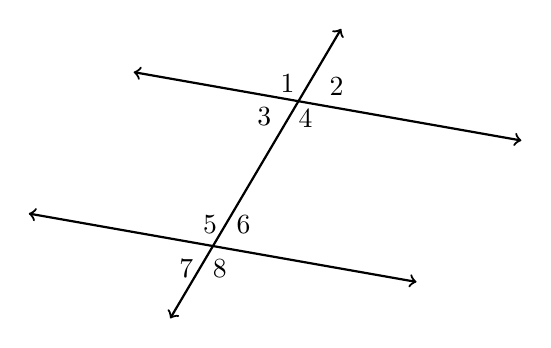
\begin{tikzpicture}[scale=1,rotate=-10]
  \draw [<->, thick] (3,2)--(8,2);
  \draw [<->, thick] (2,0)--(7,0);
  \draw [<->, thick] (4,-1)--(5.5,3);
  \node at (4.5,0.3) [left]{$5$};
  \node at (4.5,0.3) [right]{$6$};
  \node at (4.3,-0.3) [left]{$7$};
  \node at (4.3,-0.3) [right]{$8$};
  \node at (5.2,2) [above left]{$1$};
  \node at (5.4,2) [above right]{$2$};
  \node at (4.9,2) [below left]{$3$};
  \node at (5,2) [below right]{$4$};
\end{tikzpicture}
\end{flushright} 
\end{multicols} \vspace{4cm}

\item The measures in degrees of the three angles of a triangle are $2x$, $\frac{2}{5}x$, and $\frac{1}{10}x$. Find the measures of the triangle's angles. \vspace{4cm}

\newpage
\item Given $\triangle RSU$. If $m\angle UST=x+50$, $m\angle R=x-20$, and $m\angle U=x+10$, find $m\angle R$.
  \begin{flushright}
  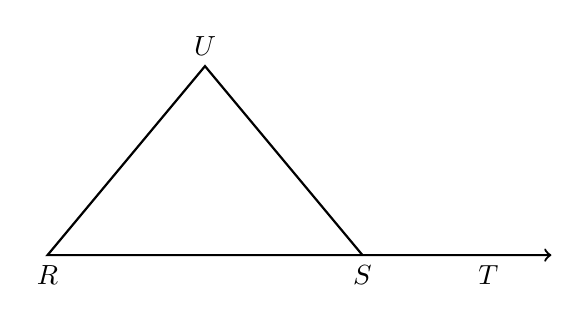
\begin{tikzpicture}[scale=0.8]
    %\draw [->, thick] (0,0)--(5,5);
    \draw [<-, thick] (8,0)--
      (7,0) node[below]{$T$}--
      (0,0) node[below]{$R$}--
      (2.5,3) node[above]{$U$}--
      (5,0) node[below]{$S$};
  \end{tikzpicture}
  \end{flushright} \vspace{2cm}

\item Given two parallel lines, two transversals
\begin{multicols}{2}
  \begin{enumerate}
    \item Find $x$, $y$
    \item What relationship are you using? \\[0.5cm]
    (e.g. vertical angles, same-side exterior angles, alternate interior angles, etc.)
  \end{enumerate}
    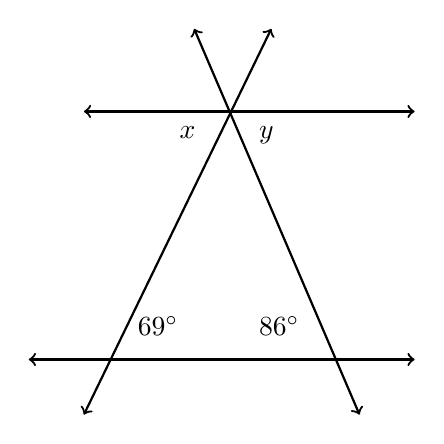
\begin{tikzpicture}[scale=1.4]
    \draw [<->, thick] (4,2.25)--(7,2.25);
    \draw [<->, thick] (3.5,0)--(7,0);
    \draw [<->, thick] (4,-0.5)--(5.7,3);
    \draw [<->, thick] (6.5,-0.5)--(5,3);
    \node at (4.4,0.3) [right]{$69^\circ$};
    \node at (5.5,0.3) [right]{$86^\circ$};
    \node at (5.1,2.2) [below left]{$x$};
    \node at (5.5,2.2) [below right]{$y$};
  \end{tikzpicture}
\end{multicols}

\item A triangle has two angles measuring $x^\circ$ and $y^\circ$ respectively. Find the measure of the third angle as an expression of $x$ and $y$. \vspace{2cm}

\newpage
\item Given  $\triangle LMN$ with $m\angle L=2x+20$, $m\angle N=3x+5$, and $m\angle M=5x+5$. Find $x$.
  \begin{flushright}
  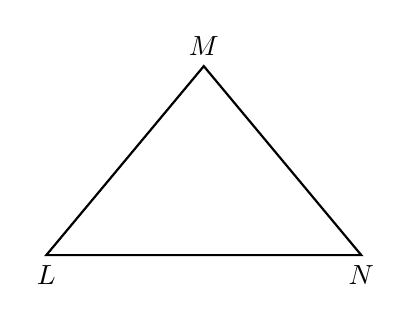
\begin{tikzpicture}[scale=0.8]
    %\draw [->, thick] (0,0)--(5,5);
    \draw [-, thick] (0,0) node[below]{$L$}--
      (2.5,3) node[above]{$M$}--
      (5,0) node[below]{$N$}--cycle;
  \end{tikzpicture}
  \end{flushright} \vspace{2cm}

\item The measures in degrees of the three angles of a triangle are $3x$, $\frac{1}{2}x+7$, and $5x-65$. Find $x$. \vspace{4cm}

\item Angles $APC$ and $CPD$ form a linear pair. $m\angle APC = 10x+15$ and $m\angle CPD = 3x-4$. Find $m\angle CPD$. Check your answer for full credit.
  \begin{flushright}
    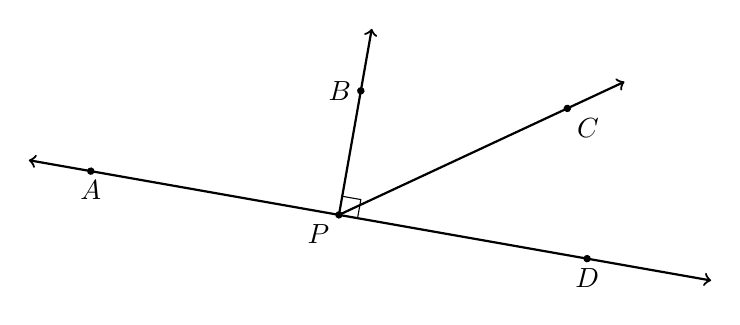
\begin{tikzpicture}[scale=0.8, rotate=-10]
      \draw [->, thick] (0,0)--(35:5);
      \draw [<->, thick] (-5,0)--(6,0);
      \draw [->, thick] (0,0)--(0,3);
      \draw (0,0)++(0.3,0)--++(0,0.3)--+(-0.3,0);
      %\draw [fill] (-1,2.5) circle [radius=0.05] node[left ]{$B$};
      \draw [fill] (35:4) circle [radius=0.05] node[below right]{$C$};
      \draw [fill] (-4,0) circle [radius=0.05] node[below]{$A$};
      \draw [fill] (0,0) circle [radius=0.05] node[below left]{$P$};
      \draw [fill] (0,2) circle [radius=0.05] node[left]{$B$};
      \draw [fill] (4,0) circle [radius=0.05] node[below]{$D$};
    \end{tikzpicture}
    \end{flushright}
    \vspace{4cm}

\end{enumerate}
\end{document}